\section{Evaluation}
\label{sec:eva}

Met een subsectie voor elke deelvraag.

In hoeverre is je vraag beantwoord?

Een mooie graphic/visualisatie is hier heel gewenst.

Hou het kort maar krachtig.

\subsection{Zijn de methodes gebruikt in \cite{state} toepasbaar op het Nederlandse troonrede corpus?}

De Nederlandse troonrede is net zoals het de Amerikaanse State of the Union een toespraak die jaarlijks vanuit de overheid worden gegeven. In beide gevallen wordt de voordracht door één positie voorgedragen, voor Nederland is dit de koning(in) en voor de VS is dit de president. Voor beide teksten geldt dat ze zijn opgebouwd uit verschillende paragrafen en er veelal voor elke paragraaf één onderwerp centraal staat. Beide hebben een centraal motief gericht op het meedelen van de huidige staat van het land en mogelijk voornemens voor het komende jaar. 
Omdat de opbouw en het doel van beide teksten zoveel op elkaar lijken zijn de methodes die gebruikt zijn binnen \cite{state} goed toepasbaar op het corpus van de Nederlandse troonredes. Hierbij hoeven er maar kleine aanpassingen gemaakt te worden, waarbij het grootste verschil ligt in het feit dat de teksten in verschillende talen zijn geschreven. Voor het Nederlands betekent gaf dit enkele problemen omdat woorden over de jaren op verschillende manieren zijn geschreven en de taal over de jaren is verandert. Zo werd het woord "de" vroeger als "den" geschreven. Hierdoor zijn enkele woorden die vroeger anders geschreven werden niet opgevangen door de POS-tagging. Op het moment dat dit duidelijk werd is het handmatig aangepast. Op deze manier is er net als in \cite{state} het corpus gereduceerd tot de relevante zelfstandige naamwoorden. Hierbij is dus gebruik gemaakt van modules die op de Nederlandse taal getraind waren. Hierna zijn de 1000 meest voorkomende termen gebruikt worden om de co-occurence matrix op te stellen dat gebruikt is om de nabijheidsscore te berekenen waarmee het semantische netwerk is gevormd.

\subsection{Zijn de resultaten representatief voor de werkelijkheid?}

De verkregen resultaten zijn de geïnduceerde onderwerpen en het daarmee verkregen overzicht van onderwerp verschuivingen. Hiervoor was het belangrijkste dat er vanuit het semantische netwerk door middel van het community clustering algoritme duidelijke clusters gevormd werden. Vanuit de termen binnen een cluster kan een achterliggend onderwerp worden bepaald dat door deze termen wordt geïmpliceerd. Het is dus noodzakelijk dat de clusters duidelijk verschillend van elkaar zijn en de relatie tussen de termen in een cluster zo min mogelijk verschillende onderwerpen impliceren. Hoe duidelijker de relatie is tussen de termen in een cluster hoe makkelijker het is om er een onderwerp aan te koppelen. Dit is het makkelijkst voor clusters die gecentreerd zijn rondom één term, zoals "onderwijs" of "ontwikkeling". 

De onderwerpen die gevonden zijn staan in tabel \ref{onderwerpen}:
\begin{table}[htb]
\centering
\begin{tabular}{ll}
\toprule
{} &                Onderwerpen \\
\midrule
 &  regeringsbeleid \\
 &        onderwijs \\
 &    arbeidsbeleid \\
 &  koloniaalbeleid \\
 &        wetgeving \\
 &     ontwikkeling \\
 &    staatplanning \\
 &         defensie \\
\bottomrule
\end{tabular}
\caption{Geïmpliceerde onderwerpen}
\label{onderwerpen}
\end{table}

Voor elk onderwerp is er een lijst met termen waarvoor geldt dat als deze voorkomen in een tekst ze dat onderwerp impliceren. Aan de hand van deze lijst is een grafiek opgesteld met daarin voor elk jaar de hoeveelheid dat een onderwerp besproken werd. Dit is gedaan door te kijken naar de volledige tekst van dat jaar en voor elk woord na te gaan bij welk onderwerp het hoort. Hierna is door gebruik te maken van een normaal verdeling een grafiek gevormd die per onderwerp procentueel aangeeft hoeveel van de troonrede besteed was aan de behandeling van dat onderwerp. Hieruit volgt de grafiek in figuur \ref{onderwerpverdeling}:

\begin{figure}[H]
\hfill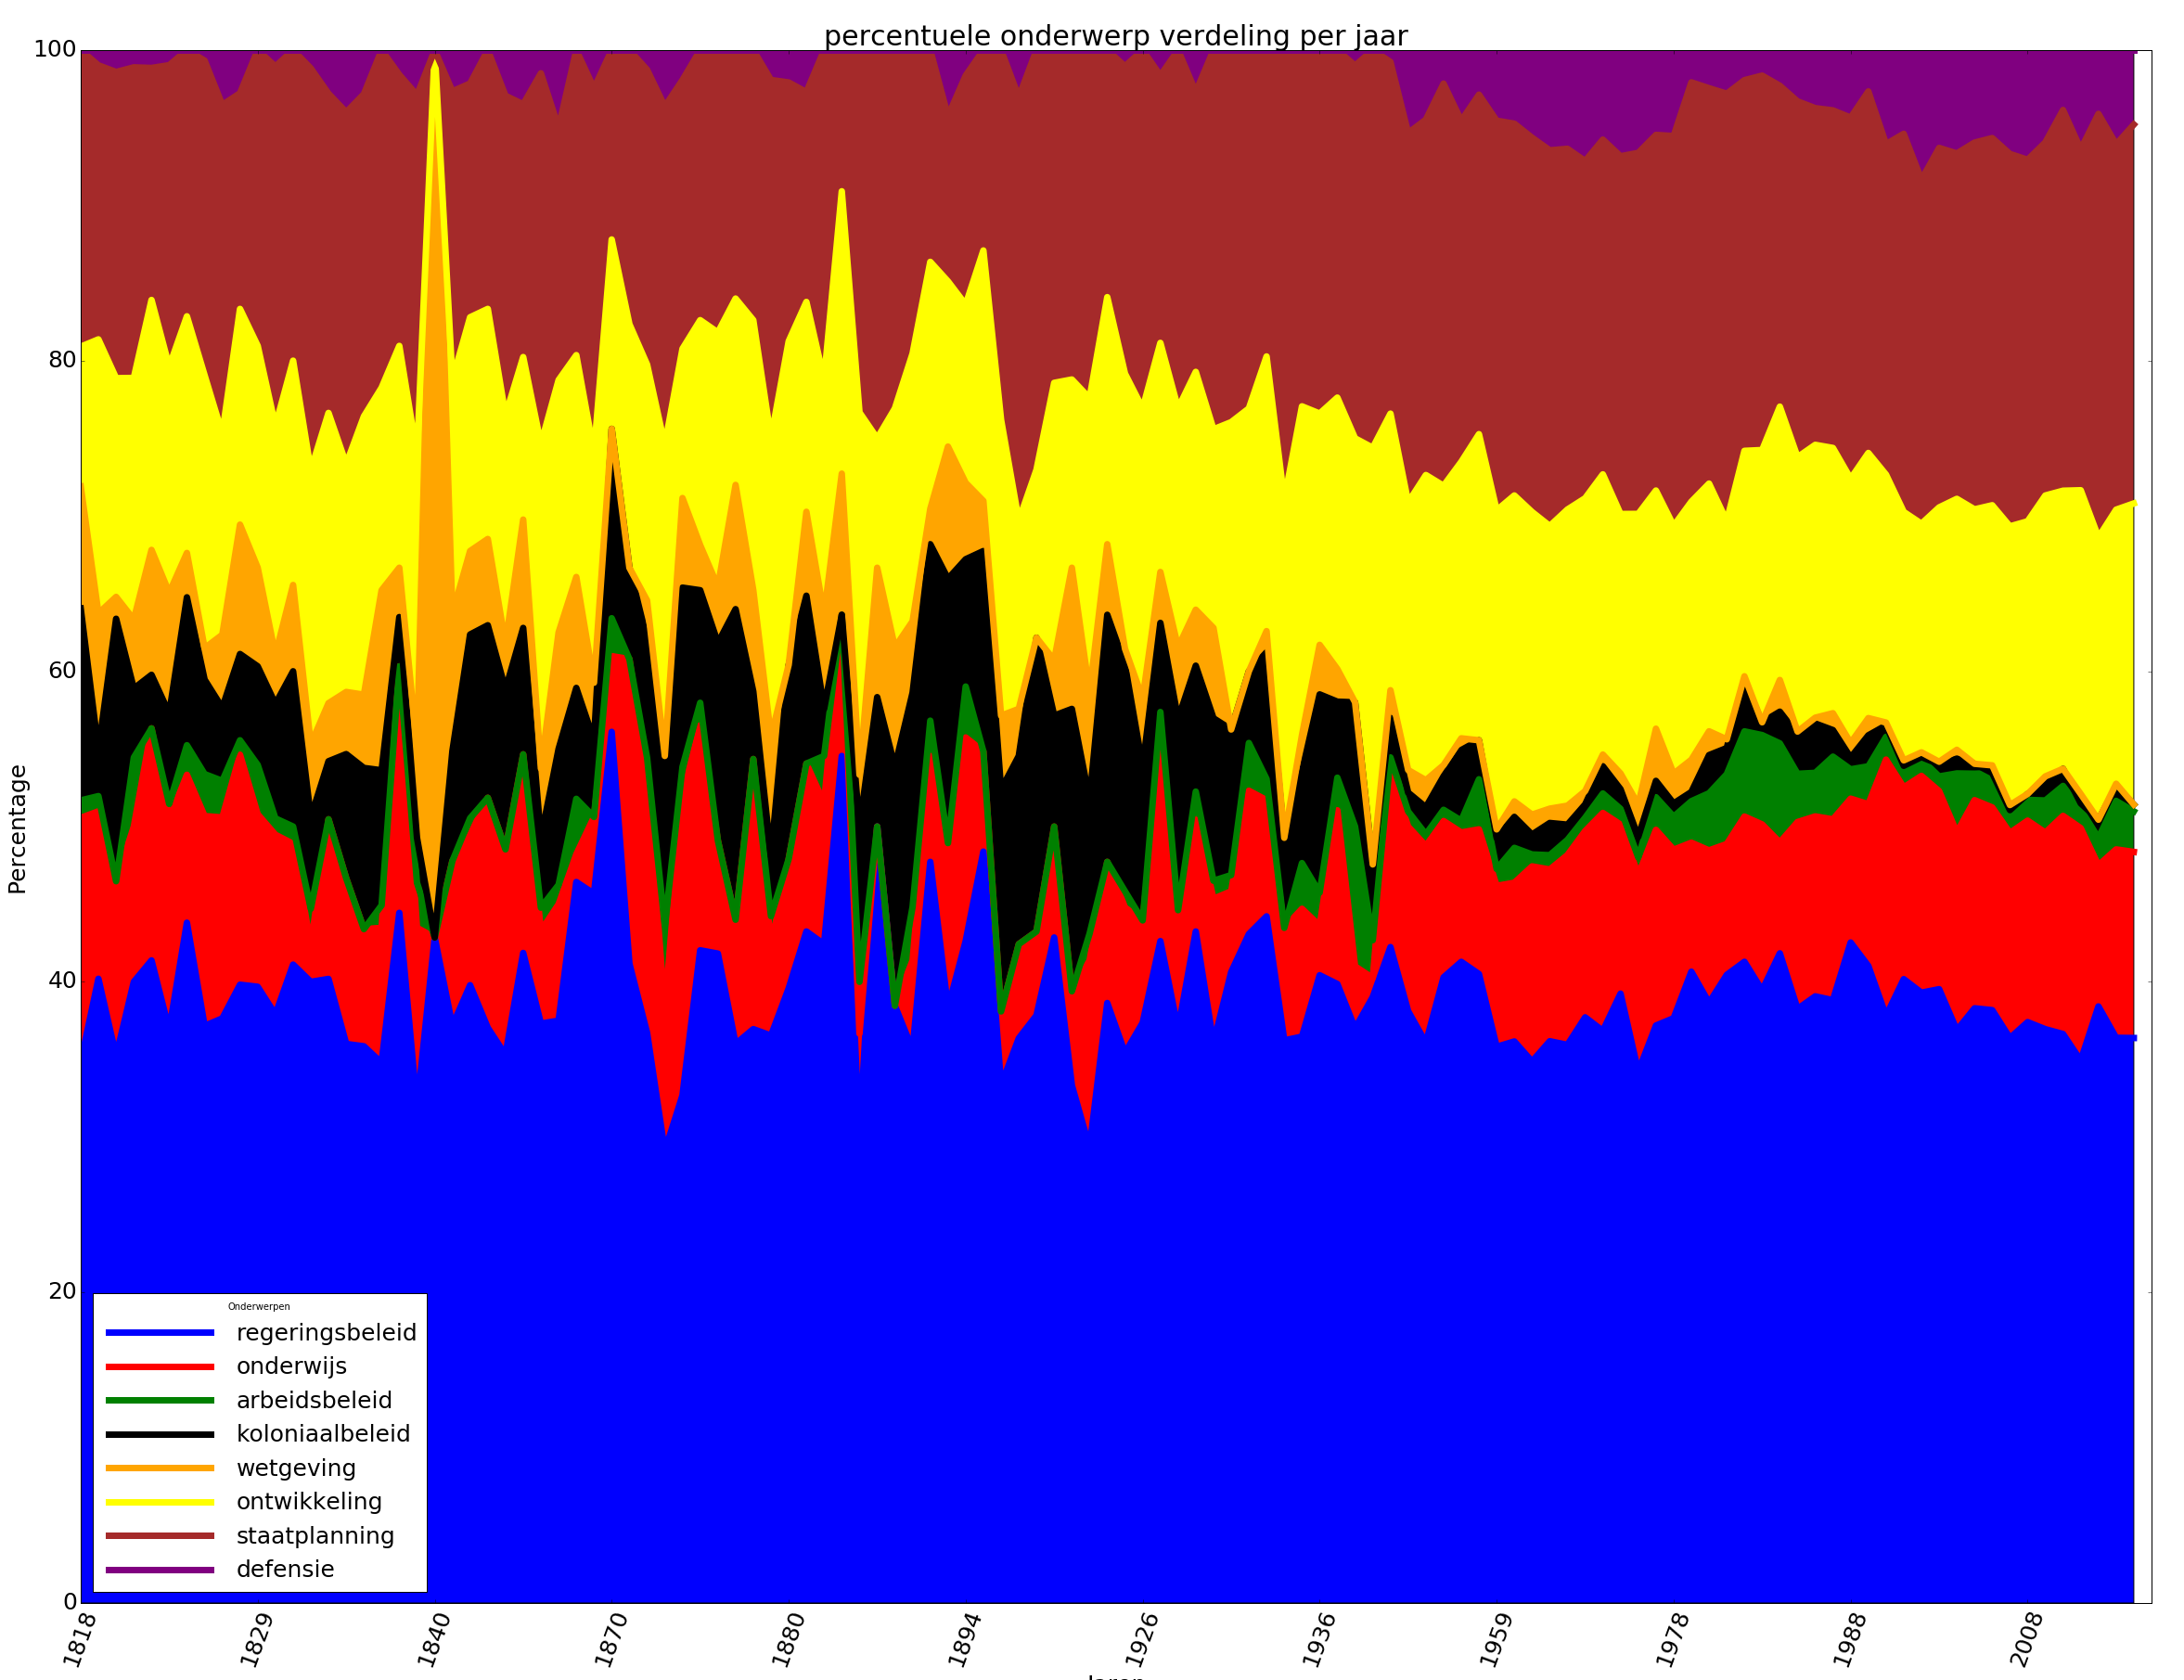
\includegraphics[width=1.2\textwidth,left]{fig/onderwerpverdeling}
\caption{\label{onderwerpverdeling} Verschuiving van inhoud van troonredes over de jaren aan de hand van de gevonden onderwerpen.}
\end{figure}


Vanuit deze grafiek is duidelijk af te lezen welke onderwerpen het belangrijkst waren in een jaar. Zo is bijvoorbeeld duidelijk te zien dat er rond 1839-40 het onderwerp wetgeving sterk naar voren komt, wat terug te leiden is naar de werkelijkheid, omdat in 1840 de officiële scheiding plaatsvond tussen Nederland en België ondertekend in het verdrag van Londen. Door dit verdrag is een groot deel van de Nederlandse grondwet aangepast. \citep{schroeder1996transformation} De resultaten zijn dus zichtbaar terug te leiden op de werkelijkheid.